\documentclass[17pt]{beamer}
%\documentclass[handout]{beamer} %Makes Handouts
\usetheme{Singapore} %Gray with fade at top
\useoutertheme[subsection=false]{miniframes} %Supppress subsection in header
\useinnertheme{rectangles} %Itemize/Enumerate boxes
\usecolortheme{seagull} %Color theme
\usecolortheme{rose} %Inner color theme

\definecolor{light-gray}{gray}{0.75}
\definecolor{dark-gray}{gray}{0.55}
\setbeamercolor{item}{fg=light-gray}
\setbeamercolor{enumerate item}{fg=dark-gray}

\setbeamertemplate{navigation symbols}{}
\setbeamertemplate{mini frames}{}
%\setbeamercovered{dynamics}
\setbeamerfont*{title}{size=\Large,series=\bfseries}
\setbeamerfont{footnote}{size=\tiny}

%\setbeameroption{notes on second screen} %Dual-Screen Notes
%\setbeameroption{show only notes} %Notes Output

\setbeamertemplate{frametitle}{\vspace{.5em}\bfseries\insertframetitle}
\newcommand{\heading}[1]{\noindent \textbf{#1}\\ \vspace{1em}}
\newcommand{\questions}{\frame{{\large Questions?}}}

\usepackage{bbding,color,multirow,times,ccaption,tabularx,graphicx,verbatim,booktabs}
\usepackage{colortbl} %Table overlays
\usepackage[english]{babel}
\usepackage[latin1]{inputenc}
\usepackage[T1]{fontenc}
\usepackage{lmodern}
\usepackage{alltt}

\usepackage{tikz}
\usetikzlibrary{shapes,arrows,decorations.pathreplacing,calc}


\author[]{Thomas J. Leeper}
\institute{
  Government Department\\London School of Economics and Political Science
}


\title{Examples and Paradigms}

\date[]{}

\begin{document}

\frame{\titlepage}

\frame{\tableofcontents}


\frame{

\frametitle{Share your TESS Examples}

With a partner, discuss 1--2 of your TESS examples
\begin{itemize}
\item What was the researcher's question?
\item How did they test it experimentally?
\item What was interesting or surprising about the designs?
\end{itemize}

Take about 4 minutes.

}



\section{From Theory to Design}
\frame{\tableofcontents[currentsection]}
% deriving hypotheses from theory and manipulations from hypotheses


\frame{

\frametitle{Experiments are good at answering ``what if'' questions}

\begin{itemize}
\item Forward causal questions
	\begin{itemize}
	\item Can X cause Y?
	\item What effects does X have?
	\end{itemize}
\item<2-> Backward causal questions
	\begin{itemize}
	\item What causes Y?
	\item How much of Y is attributable to X?
	\end{itemize}
\end{itemize}
}



\frame{

\frametitle{What makes a good research question?}

KKV's two criteria:

\begin{enumerate}
\item Politically important
\item Contribute to scientific understanding/literature
\vspace{0.5em}
\item<2-> Personally interesting
\item<2-> Unresolved
\item<3-> For experiments, forward in nature
\end{enumerate}
}

\frame{

Even though answering ``forward'' causal question, we start with an outcome concept.

\begin{itemize}
\item Term/label
\item Attributes (i.e., definition)
\item Indicators (i.e., operationalization)
\end{itemize}

% ACTIVITY

}


\frame{

We may have a "big" theory (like the effect of democratization on economic growth).

This isn't particularly well-suited to experimental intervention for various reasons (cost, ethics, finite population of countries, etc.), but there are possibly causal mechanisms or empirical implications that could be tested.

E.g., we can design an experiment where some citizens are invited to deliberate with authoritarian rulers on a local level (while a control group is not invited to participate) and then compare their economic productivity


}


\frame{

\frametitle{Hypotheses}


\begin{itemize}
\item From theory, we derive testable hypotheses
\item Hypotheses are expectations about differences in outcomes across levels of a putatively causal variable
\end{itemize}


% ACTIVITY

}


\frame{

\begin{itemize}
\item Derive experimental design from hypotheses
\item We can only test hypotheses by comparing two (or more) experimental conditions
\item Experimental ``factors'' are expressions of hypotheses as randomized groups
\item What intervention each group receives depends on hypotheses
	\begin{itemize}
	\item presence/absence
	\item levels/doses
	\item qualitative variations
	\end{itemize}
\end{itemize}

}


% Talk about protocol and preregistration

\frame{

\frametitle{Protocol}

Protocol\footnote{Thomas J. Leeper. 2011. ``The Use of Protocol in the Design and Reporting of Experiments.'' \textit{The Experimental Political Scientist}.} is the complete planning document for how to design, implement, and analyze an experiment

It contains details of:

\begin{enumerate}
\item Theory/hypotheses
\item Instrumentation
	\begin{itemize}
	\item Manipulation(s)
	\item Outcome(s)
	\item Covariate(s)
	\item Manipulation check(s)
	\end{itemize}
\item Sampling
\item Implementation
\item Analysis
\end{enumerate}
}

\frame{

\frametitle{Activity!}

\begin{itemize}
\item With a partner, identify each of the protocol elements of the experiment described by Kahneman and Tversky
\begin{enumerate}
\item Theory/hypotheses
\item Instrumentation
\item Sampling
\item Implementation
\item Analysis
\end{enumerate}
\item Report back in about 7 minutes
\end{itemize}

}


\subsection{Question Wording Designs}
\frame{\tableofcontents[currentsubsection]}

\frame{

\frametitle{Question Wording Designs}

\begin{itemize}
\item Kahneman and Tversky is ``question wording'' experiment
\item Hypothesized difference in outcomes according to the decision being faced
	\begin{itemize}
	\item Risky or not risky
	\item Gains or losses
	\end{itemize}
\item Manipulation operationalizes this by asking two different questions
\item Outcome is the answer to the question
\end{itemize}

}


\frame{

\frametitle{``Framing'' Experiments}

\begin{itemize}
\item Example: Schuldt et al. ```Global Warming' or `Climate Change'? Whether the Planet is Warming Depends on Question Wording.''

\end{itemize}
}

\frame{

\frametitle{Subtle Cue Experiments}

}

\frame{

\frametitle{Question testing}

Use question wording designs to select which survey measures we want to use

\begin{itemize}
\item Select possible question wordings
\item Select some criterion(-ia) for assessing which is better
\item Pilot test and then use the item that performs better
\end{itemize}

}

\frame{

\vspace{-1em}
\footnotesize
    \begin{columns}[T]
    \begin{column}[T]{5cm}
        \begin{block}{}
            In talking to people about elections, we often find that a lot of people were not able to vote because they weren't registered, they were sick, or they just didn't have time. How about you--did you vote in the elections this November?
        \end{block}
    \end{column}
    \begin{column}[T]{5cm}
        \begin{block}{}
            In talking to people about elections, we often find that a lot of people were not able to vote because they weren't registered, they were sick, or they just didn't have time. Which of the following statements best describes you?
            \vspace{-1em}
            \begin{itemize}\itemsep-0.2em\tiny
            \item One, I did not vote in the November 3 election
            \item two, I thought about voting this time but didn't
            \item three, I usually vote but didn't this time
            \item four, I am sure I voted
            \end{itemize}
        \end{block}
    \end{column}
    \end{columns}
}




\subsection{Assessing Treatments}
\frame{\tableofcontents[currentsubsection]}


% manipulation checks: Manipulation checks are a measurement of our manipulated variable
% pretesting

\frame{

\frametitle{How do we know we manipulated what we think we manipulated?}
\begin{itemize}
\item<2-> Outcomes are affected consistent with theory
\item<3-> Before the study using \textit{pilot testing} (or \emph{pretesting})
\item<4-> During the study, using \emph{manipulation checks}
\item<5-> During the study, using \textit{non-equivalent outcomes}
\end{itemize}
}

\frame{

\frametitle{I. Outcomes Affected}

\begin{itemize}
\item Tautological!
\item Doesn't tell us anything if we hypothesize null effects
\end{itemize}

}


\frame{

\frametitle{II. Pilot Testing}

\begin{itemize}
\item Like question wording, but assess whether a set of possible manipulations affect a measure of the \textit{independent} variable
\item<2-> Example:
	\begin{itemize}
	\item Goal: Manipulate the ``strength'' of an argument
	\item Write several arguments
	\item Ask pilot test respondents to report how strong each one was
	\end{itemize}
\end{itemize}

}

\frame{

\frametitle{III. Manipulation Checks}

\begin{itemize}
\item Measures added post-treatment, post-outcome that assess whether the \textit{independent} variable was affected by treatment
\item<2-> Example:
	\begin{itemize}
	\item Goal: Manipulate whether respondent believes a policy is expensive or not
	\item Outcome is support for the policy
	\item Manipulation check comes after opinion question, asking how expensive the respondent believes policy is
	\item Compare beliefs in treatment and control conditions
	\end{itemize}
\end{itemize}

}

\frame{

\frametitle{IV. Non-equivalent outcomes}

\begin{itemize}
\item Measures an outcome that \textit{should not} be affected by independent variable
\item<2-> Example:
	\begin{itemize}
	\item 
	\end{itemize}
\end{itemize}

}


\subsection{Question Order Designs}
\frame{\tableofcontents[currentsubsection]}

\frame{

\frametitle{Question Order Designs}

\begin{itemize}
\item Manipulation comes in the order or set of questions before the outcome measure
\item<2-> Example:
	\begin{itemize}
	\item Goal: assess influence of value salience on support for a policy
	\item Manipulate salience by asking different questions:
		\begin{itemize}
		\item Battery of 5 ``individual liberties'' questions, or
		\item Battery of 5 ``life'' questions
		\end{itemize}
	\item Measure support for legalized abortion
	\end{itemize}
\item<3-> If answers to manipulated questions are important, can measure rest of battery post-outcome
\end{itemize}

}



\subsection{Vignette Designs}
\frame{\tableofcontents[currentsubsection]}

% vignette
% text
% video

\subsection{Sensitive Item Designs}
\frame{\tableofcontents[currentsubsection]}





\section{Surveys in Larger Designs}
\frame{\tableofcontents[currentsection]}

% quasi-experiments and field experiments


\frame{

\frametitle{Field Designs}

\begin{itemize}
\item Surveys can be used as a measurement instrument for a field treatment
\item No manipulation in the survey itself
\item Survey only measures outcomes post-treatment
\item Common uses:
	\begin{itemize}
	\item Randomized treatment
	\item Quasi-experimental treatment
	\item Timing treatment
	\end{itemize}
\end{itemize}

}


\frame{

\frametitle{Randomized Treatment}

% compliance problems
% non-response problems

}


\frame{

\frametitle{Quasi-Experimental Treatment}

}


\frame{

\frametitle{Timing Treatment}

}





\frame{

	\frametitle{Threats to Validity}
	\begin{enumerate}
	\item History
	\item Maturation
	\item Testing
	\item Instrumentation
	\item Instability
	\item Regression to the mean
	\end{enumerate}
}
% history: stimultaneous alterntive cause
% maturation: time trends
% testing: measurement changes behavior
% instrumentation: operationalization changes over time
% instability: measurement error
% regression (to the mean):
% - statistically: extreme cases will be less extreme on second measurement
% - in policy terms: interventions are most likely when problems are extreme

% one more not mentioned by Campbell and Ross: If the series is an aggregation, it's also possibly due to attrition or changing composition of the sample from which the data is aggregated

\frame{
	\frametitle{Difference-In-Differences}
	\small
	\begin{itemize}\itemsep0.5em
		\item How do we know change in $Y$ wasn't due to something else?
			\begin{itemize}
				\item How do we know $Y_{0,t}$ is a good stand-in for $Y_{0,t+1}$?
			\end{itemize}
		\item<2-> Use a comparison case (or cases)!
		\item<3-> Instead of using the pre-post difference in $Y_i$ to estimate the causal effect, use the difference in pre-post differences for two units $i$ and $j$:
		\begin{align*}
		(Y_{i,t+1} - Y_{i,t}) - (Y_{j,t+1} - Y_{j,t})
		\end{align*}
	\end{itemize}
}


\frame{
	\begin{center}
	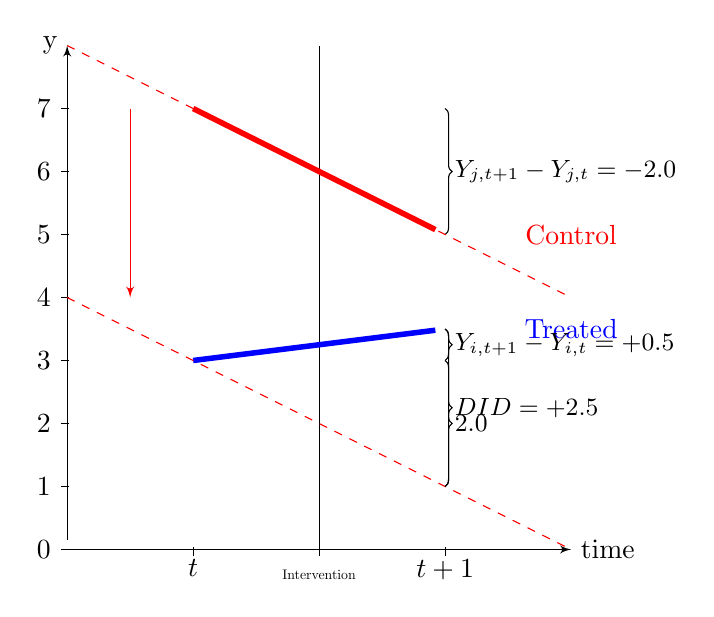
\begin{tikzpicture}[>=latex', scale=0.8]
        \draw[->] (0,0) node (origin) {}  -- (8,0) node[right] (xaxis) {time};
        \draw[->] (origin) -- (0,8) node[left] (yaxis) {y};
        % x ticks
        \foreach \x in {2,4,6}
        	\draw (\x,1pt) -- (\x,-3pt) node[anchor=north] {};
        \draw (2,0) node[below] (before) {$t$};
        \draw (6,0) node[below] (after) {$t+1$};
        \draw (4,-0.25) node[below, scale=0.5] (IV) {Intervention};
        % y ticks
        \foreach \y in {0,...,7}
             \draw (1pt,\y) -- (-3pt,\y) node[anchor=east] {$\y$};
        % intervention
        \draw (4,0) -- (4,8);

        % line
        \draw<2-> (6,3.5) node (tr) {};
        \draw<3-> (6,5) node (ctrl) {};
        \draw<2-3>[blue] (8,3.5) node (trlab) {Treated};
        \draw<3-3>[red] (8,5) node (ctrllab) {Control};        
        \draw<2->[blue, line width=2pt] (2,3) -- (tr);
        \draw<3->[red, line width=2pt] (2,7) -- (ctrl);
        
        % diffs
        \draw<4-6>[right,decorate,decoration={brace,mirror}] 
        	(6,3) -- (6,3.5) node[right, pos=0.5] (idiff) {\small $Y_{i,t+1} - Y_{i,t} = +0.5$};
        \draw<4-6>[right,decorate,decoration={brace}] 
            (6,7) -- (6,5) node[right, pos=0.5] (jdiff) {\small $Y_{j,t+1} - Y_{j,t} = -2.0$};
        
        % trends
        \draw<5-6>[red,->] (1,7) -- (1,4);
        \draw<5->[red, dashed] (0,8) -- (8,4);
        \draw<5->[red, dashed] (0,4) -- (8,0);
        \draw<6>[right,decorate,decoration={brace}] 
            (6,3) -- (6,1) node[right, pos=0.5] (idiff2) {\small $2.0$};
        \draw<7>[right,decorate,decoration={brace}] 
            (6,3.5) -- (6,1) node[right, pos=0.5] (idiff2) {\small $DID = +2.5$};
                        
        
    \end{tikzpicture}
    \end{center}
}




\frame{
	\frametitle{What is a Quasi-Experiment?}
	\small
	\begin{itemize}\itemsep0.5em
		\item Quasi-Experiments are situations where randomization-like forces influence the values of independent variables
		\item Most of the time, these are ``natural'' experiments where boundaries, discontinuities, or interruptions disrupt a continuous treatment-assignment process
		\item Analyzing a quasi-experiment involves searching for an ``instrument variable''
	\end{itemize}
}


\frame{
	\frametitle{What is ``instrumental''?}
	\begin{enumerate}\itemsep0.5em
		\item \alert<2>{serving as a crucial means, agent, or tool}
		\item of, relating to, or done with an instrument or tool
		\item relating to, composed for, or performed on a musical instrument
		\item of, relating to, or being a grammatical case or form expressing means or agency
	\end{enumerate}
}



\frame{
	\frametitle{What is ``instrumental''?}
	\begin{itemize}\itemsep1em
		\item $W$ must be a crucial cause of $X$'s effect on $Y$
		\item $W$ is the quasi-experimental shock to the causal process in our graph
			\begin{itemize}
			\item It is not caused by $X$ or $Y$
			\item It does not cause $Y$ except through $X$
			\end{itemize}
	\end{itemize}	
}

\frame{
	\frametitle{Formal Definition}
	An \textbf{instrumental variable} is a variable that satisfies two properties:\\
	\begin{enumerate}\itemsep0.5em
		\item Exogeneity\\ % Not testable
			\begin{itemize}
				\item $W$ temporally precedes $X$
				\item $Cov(B, \epsilon) = 0$
			\end{itemize}
		\item Relevance\\ % Is testable
			\begin{itemize}
				\item $W$ causes $X$
				\item $Cov(W, X) \neq 0$
			\end{itemize}
	\end{enumerate}
}



\frame{
	\frametitle{How IV Works I}
	\begin{itemize}\itemsep0.5em
		\item Start with case where $W$ is 0,1
		\item To identify the effect $X \rightarrow Y$, all we need is $W$
		\item We don't need to worry about other omitted variables, but we don't learn anything about the rest of the causal graph
	\end{itemize}
}

\begin{frame}
\small 
\begin{center}
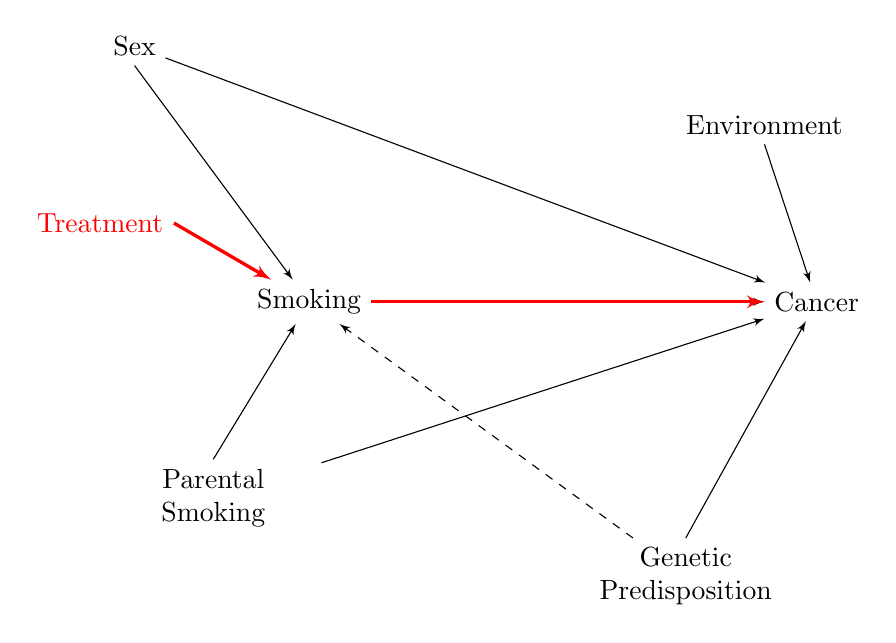
\begin{tikzpicture}[>=latex',circ/.style={draw, shape=circle, node distance=5cm, line width=1.5pt}]
    \draw[->] (0,0) node[left] (X) {Smoking} -- (5,0) node[right] (Y) {Cancer};
    \draw[->] (-3,3) node[above] (Z) {Sex} -- (X);
    \draw[->] (Z) -- (Y);
    \draw[->] (5,2) node[above] (A) {Environment} -- (Y);
    \draw[->] (4,-3) node[below, text width=3cm, align=center] (E) {Genetic\\Predisposition} -- (Y);
    \draw[->] (-2, -2) node[below, text width=2.5cm, align=center] (W) {Parental\\Smoking} -- (X);
    \draw[->] (W) -- (Y);
    \draw[->, dashed] (E) -- (X);
    
    \draw[->, very thick, color=red] (-2.5,1) node[left, color=red] (Tr) {Treatment} -- (X);
    \draw[->, very thick, color=red] (X) -- (Y);
\end{tikzpicture}
\end{center}
\end{frame}

\frame{
	\frametitle{How IV Works II (Wald)}
	\small
	\begin{itemize}\itemsep0.5em
		\item Imagine two effects:
		\begin{align}
		ITT_y & = E[y_i | w_i = 1] - E[y_i | w_i = 0]\\
		ITT_x & = E[x_i | w_i = 1] - E[x_i | w_i = 0]
		\end{align}
		\item IV estimates the LATE: $\dfrac{ITT_y}{ITT_x}$
		\item In a regression, this is:\\
			$E[y_i|w_i] = \beta_0 + \text{LATE} \times E[x_i|w_i]$
	\end{itemize}
}


\frame{
	\frametitle{{\large Local Average Treatment Effect}}
	\small
	\begin{itemize}\itemsep0.5em
	\item IV estimate \textit{local} to the variation in $X$ that is due to variation $W$ (i.e., the LATE)
	\item This matters if effects are \textit{heterogeneous}
	\item LATE is effect for those who \textit{comply} with instrument
	\item Four subpopulations:
		\begin{itemize}\small
		\item Compliers: $X = 1$ only if $W = 1$
		\item Always-takers: $X = 1$ regardless of $W$
		\item Never-takers: $X = 0$ regardless of $W$
		\item Defiers: $X = 1$ only if $W = 0$
		\end{itemize}
	\end{itemize}
}




\frame{
	\frametitle{Finding Instruments}
	\begin{itemize}\itemsep0.5em
		\item Forward, not backward, causal inference
		\item Most instruments are not things we care about
			\begin{itemize}
				\item Weather, disasters
				\item Geography, borders, climate
				\item Lotteries
			\end{itemize}
		\item A good instrument is one that satisfies both of our conditions, so we need:
			\begin{itemize}
				\item A good story about exogeneity
				\item Evidence that instrument is \textit{strong}
			\end{itemize}
	\end{itemize}
}





\frame{

\frametitle{Homework!}

\begin{itemize}
\item 
\end{itemize}

}



\appendix
\frame{}

\end{document}
